\documentclass[../Dokumentacja.tex]{subfiles}
\begin{document}
\subsection{Użytkownik}
Użytkownik jest jest osobą obsługującą The Project Game.
Inicjuje wszystkie moduły. Posiada wymienione poniżej możliwości ingerencji
w działanie poszczególnych modułów.
\subsubsection{Moduł Serwera Komunikacyjnego}
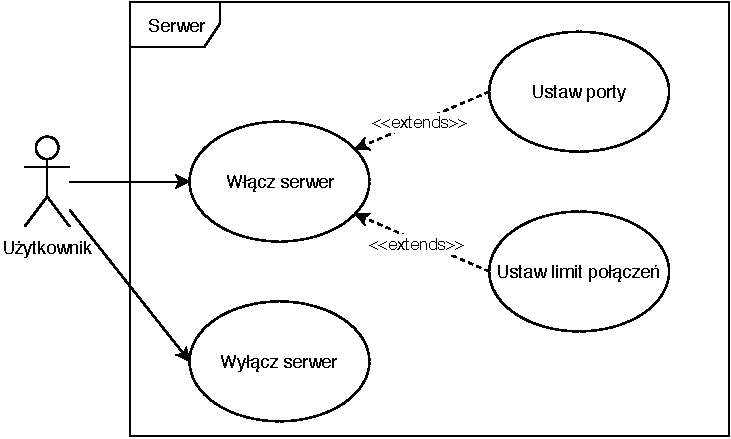
\includegraphics[width=\textwidth]{resources/USER-SERVER.pdf}

\begin{itemize}
    \item Włączanie serwera
    \begin{itemize}
    	\item Ustawianie portów do połączeń z GM oraz agentami
    	\item Ustawianie limitu ilości połączeń
    \end{itemize}
    \item Wyłączanie serwera w dowolnym momencie
\end{itemize}

\subsubsection{Moduł agenta}
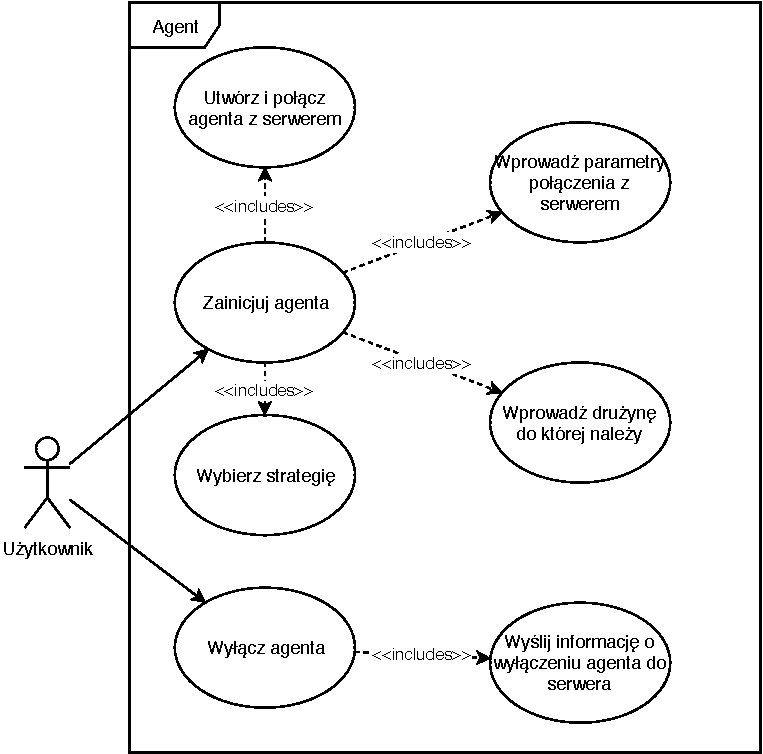
\includegraphics[width=\textwidth]{resources/USER-AGENT.pdf}
\begin{itemize}
	\item Inicjowanie agenta
	\begin{itemize}
		\item Zainicjowanie agenta wymaga parametrów połączenia z Serwerem Komunikacyjnym
		\item Wyspecyfikowanie do której drużyny należy agent (Red, Blue)
		\item Wybranie strategii używanej podczas gry przez agenta spośród zaimplementowanych w module agenta. Od wybranej strategii zależy sposób podejmowania przez agenta takich decyzji jak: przesunięcie się na planszy, opuszczenie fragmentu, czy odpowiedź innemu agentowi na zapytanie. Wybór strategi sprowadza się do wybranie identyfikatora strategii spośród specyfikowanych przez konkretnego agenta.
	\end{itemize}
	\item Wyłączanie agenta
	\begin{itemize}
		\item Agenta można wyłączyć w każdym momencie, nie ma to wpływu na przebieg rozgrywki w której uczestniczył.
	\end{itemize}
\end{itemize}

\subsubsection{Moduł GM}
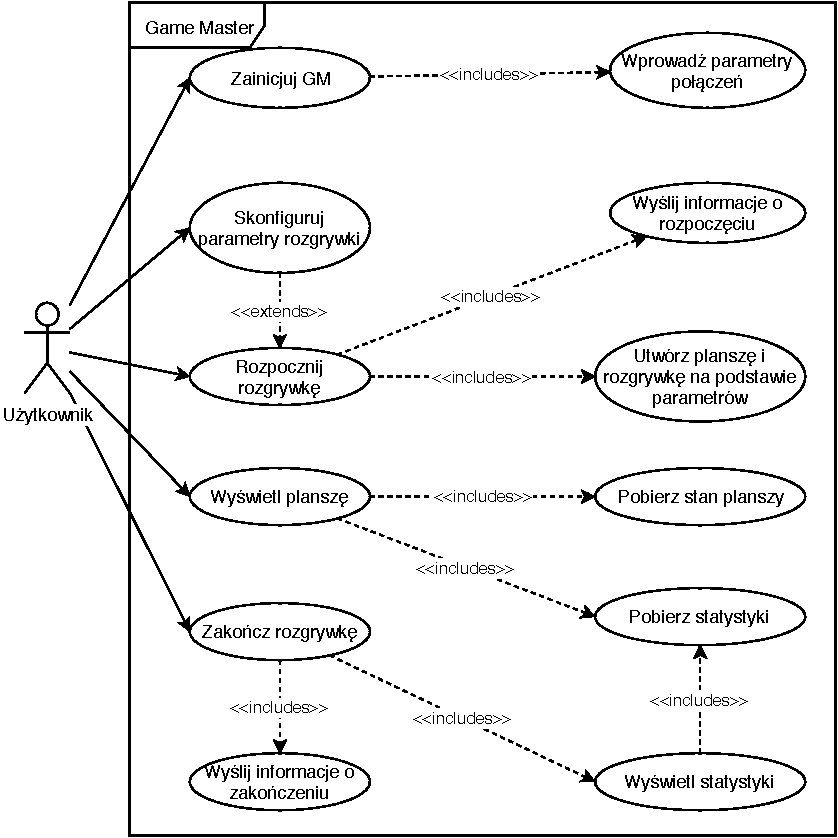
\includegraphics[width=\textwidth]{resources/USER-GM.pdf}
\begin{itemize}
	\item Inicjowanie GM
	\begin{itemize}
		\item Zainicjowanie GM wymaga wprowadzanie parametrów połączeń
	\end{itemize}
	\item Użytkownik ma możliwoś skonfigurowania parametrów rozgrywki, przed jej rozpoczęciem
	\begin{itemize}
		\item Ilość celów w polu bramkowym
		\item Wymiary pola bramkowego
		\item Opóźnienie w wykonywaniu ruchów przez agenta
		\item Wymiary planszy
		\item Maksymalna ilość agentów
		\item Prawdopodobieństwo, że pojawiający się fragment jest fragmentem fikcyjnym
		\item Częstotliwość generowania nowego fragmentu na planszy
	\end{itemize}
	\item Rozpoczynanie rozgrywki
	\begin{itemize}
		\item Użytkownik może zarządać rozpoczęcia rozgrywki, od tego momentu GM przechodzi w stan wyświetlania planszy i nie możliwa jest zmiana kofiguracji rozgrywki.
	\end{itemize}
	\item Wyświetlanie planszy
	\begin{itemize}
		\item Wyświetlenie graficznej interpretacji aktualnego stany gry. Na widoku znajduje się mapa z rozmieszeniem pól, Agetnów i fragmetów i podstawowe statystyki rozgrywki.
	\end{itemize}
	\item Zakończenie rozgrywki
	\begin{itemize}
		\item W dowolnym momencie trwającej rozgrywki użytkownik może zażądać zakończenia jej. Żądanie te przekierowuje na ekran z statystykami rozgrywki po czym kończy działanie GM
	\end{itemize}
\end{itemize}
\end{document}
